\pdfoutput=1
% Options for packages loaded elsewhere
\PassOptionsToPackage{unicode}{hyperref}
\PassOptionsToPackage{hyphens}{url}
\PassOptionsToPackage{dvipsnames,svgnames,x11names}{xcolor}
\documentclass[
  11pt,
]{article}
\usepackage{xcolor}
\usepackage[margin=1in]{geometry}
\usepackage{amsmath,amssymb}
\setcounter{secnumdepth}{-\maxdimen} % remove section numbering
\usepackage{iftex}
\ifPDFTeX
  \usepackage[T1]{fontenc}
  \usepackage[utf8]{inputenc}
  \usepackage{textcomp} % provide euro and other symbols
\else % if luatex or xetex
  \usepackage{unicode-math} % this also loads fontspec
  \defaultfontfeatures{Scale=MatchLowercase}
  \defaultfontfeatures[\rmfamily]{Ligatures=TeX,Scale=1}
\fi
\usepackage{lmodern}
\ifPDFTeX\else
  % xetex/luatex font selection
\fi
% Use upquote if available, for straight quotes in verbatim environments
\IfFileExists{upquote.sty}{\usepackage{upquote}}{}
\IfFileExists{microtype.sty}{% use microtype if available
  \usepackage[]{microtype}
  \UseMicrotypeSet[protrusion]{basicmath} % disable protrusion for tt fonts
}{}
\makeatletter
\@ifundefined{KOMAClassName}{% if non-KOMA class
  \IfFileExists{parskip.sty}{%
    \usepackage{parskip}
  }{% else
    \setlength{\parindent}{0pt}
    \setlength{\parskip}{6pt plus 2pt minus 1pt}}
}{% if KOMA class
  \KOMAoptions{parskip=half}}
\makeatother
\usepackage{longtable,booktabs,array}
\newcounter{none} % for unnumbered tables
\usepackage{calc} % for calculating minipage widths
% Correct order of tables after \paragraph or \subparagraph
\usepackage{etoolbox}
\makeatletter
\patchcmd\longtable{\par}{\if@noskipsec\mbox{}\fi\par}{}{}
\makeatother
% Allow footnotes in longtable head/foot
\IfFileExists{footnotehyper.sty}{\usepackage{footnotehyper}}{\usepackage{footnote}}
\makesavenoteenv{longtable}
\usepackage{graphicx}
\makeatletter
\newsavebox\pandoc@box
\newcommand*\pandocbounded[1]{% scales image to fit in text height/width
  \sbox\pandoc@box{#1}%
  \Gscale@div\@tempa{\textheight}{\dimexpr\ht\pandoc@box+\dp\pandoc@box\relax}%
  \Gscale@div\@tempb{\linewidth}{\wd\pandoc@box}%
  \ifdim\@tempb\p@<\@tempa\p@\let\@tempa\@tempb\fi% select the smaller of both
  \ifdim\@tempa\p@<\p@\scalebox{\@tempa}{\usebox\pandoc@box}%
  \else\usebox{\pandoc@box}%
  \fi%
}
% Set default figure placement to htbp
\def\fps@figure{htbp}
\makeatother
\setlength{\emergencystretch}{3em} % prevent overfull lines
\providecommand{\tightlist}{%
  \setlength{\itemsep}{0pt}\setlength{\parskip}{0pt}}
\usepackage{xurl}
\usepackage{etoolbox}
\AtBeginEnvironment{longtable}{\small}
\usepackage{caption}
\captionsetup{font=small,justification=raggedright}
\usepackage{bookmark}
\IfFileExists{xurl.sty}{\usepackage{xurl}}{} % add URL line breaks if available
\urlstyle{same}
\hypersetup{
  pdftitle={What should an agent carry between ARC-AGI-3 levels? Verbatim plans complete none of 1{,}186 next-level replays},
  pdfauthor={Carson Rodrigues},
  colorlinks=true,
  linkcolor={black},
  filecolor={Maroon},
  citecolor={Blue},
  urlcolor={blue},
  pdfcreator={LaTeX via pandoc}}

\title{What should an agent carry between ARC-AGI-3 levels? Verbatim
plans complete none of 1,186 next-level replays\thanks{An earlier
version of this paper was submitted to the ARC Prize 2026 Paper Track on
Kaggle.}}
\author{Carson Rodrigues}
\date{November 2026}

\begin{document}
\maketitle
\begin{abstract}
ARC-AGI-3 games reuse and extend their mechanics across levels and
change their layout, so an agent that has solved level \(k\) holds two
things it could reuse on level \(k{+}1\): the \textbf{plan} it used, or
the \textbf{mechanics} it learned. Entries carry a plan, a rule or both
from level to level, and none we found measures which helps on hidden
games. We measure which transfers, three ways: in the 340 released human
replay sessions, in a controlled ablation of our own agent, and in
paired hidden-set draws of a large language model (LLM) harness with its
\texttt{solved\_levels()} helper on and off. Replayed verbatim from the
moment level \(k\) ends, a winning sequence completes the next level in
0 of 1,186 testable pairs (23 games with a working positive control, 144
distinct level transitions, so a 95 percent upper bound of 2.5 percent;
control 99.7 percent). In the 452 of those pairs where the sequence is
at least as long as the next human solution it also completes none (113
distinct transitions, upper bound 3.2 percent). Successive winning
sequences are only slightly more alike than a shuffle (0.446 against
0.431; difference 0.015, session-cluster 95 percent interval 0.012 to
0.019). A mechanics model predicts the next level's movement at 0.740
(pair mean over 10 movement games; session-cluster 95 percent interval
0.687 to 0.791) against a 0.301 null, short of our 0.8 bar. The harness
comparison is too coarse to confirm or refute anything: two hidden draws
per arm average 24.65 with the helper and 27.89 without, a 3.2-point gap
inside the 11 points the design resolves. For our own agent, one hidden
draw per arm is consistent with a hidden metric that rewards first-level
efficiency and barely registers later-level coverage.
\end{abstract}

\section{1. The question}\label{the-question}

ARC-AGI-3 {[}1{]} is an interactive benchmark of turn-based games. In
each, an agent sees a 64 by 64 grid of 16 colours, is told neither the
goal nor the mechanics, and must clear a sequence of levels. The report
lists 25 public games and two private hold-out sets of 55 games each;
the Kaggle competition reruns a submitted notebook on its 110 hidden
games, 55 of which score the public leaderboard (the ``hidden 55''
below) and the other 55 decide the final ranking. The benchmark scores
agents by RHAE, relative human action efficiency. In the technical
report {[}1{]}, a completed level earns
\(100 \times \min(1.15, (\text{human actions} / \text{agent actions})^2)\),
weighted by level number. Squaring the ratio rewards efficiency far more
than coverage, so clearing many levels slowly earns almost nothing.
Level 1 is bounded below by discovery; later levels are where an agent
can be cheap, and only if something it holds still applies. The question
is what to carry across levels.

\section{2. Prior work}\label{prior-work}

Entries fall into three families. Harnesses let a language model work in
a Python read-eval-print loop (REPL) against the game frames: the Duck
{[}2{]} and Franzen's Milestone-2 solution {[}3{]}. Franzen's level-up
prompt tells the model to plan afresh and reuse the previous level's
mechanics; rellik13's fork {[}4{]} pins each cleared level's rule and
last 30 winning actions. StochasticGoose {[}5{]} is a convolutional
neural network (CNN) that predicts whether an action changes the frame
and resets at each level. Some notebooks {[}6{]} search the public
games' source, which the hidden games do not expose. Papers report RHAE
of 93 to 100 on the 25 public games with their best frontier-model
configurations (Tycho {[}7{]}, Twin {[}8{]}, PRO-LONG {[}9{]}, Schema
{[}10{]}, VISTA {[}11{]}, Memento 3 {[}12{]}, Kepler {[}13{]}), a set
that the study introducing AERA, the Adaptive Epistemic Reasoning Agent
{[}14{]}, finds reachable by non-intelligent strategies. The memory
ablations we found are on public games: PRO-LONG gains 18.0 points on
average across frontier models over a baseline agent without its log,
NVIDIA's Object-Oriented Agents (NOOA) {[}15{]} 11.8 over plain markdown
files, and Tracing {[}16{]} finds that scripts an agent writes for one
task are almost never called on a later one (33 of 630 references cross
a task boundary; a task there is a level). We found no paired hidden-set
comparison of what to carry across levels (a web search with three
queries on 30 October 2026, and an arXiv search for ``ARC-AGI-3'' on 2
November 2026 that returned 31 papers, screened by abstract; not a
systematic review). Two October preprints read in full use only the
public games: Lencevicius {[}17{]} varies what a harness carries between
turns (dropped turns, summaries, a note-taking instruction, replayed
reasoning) for one model on four games, and Liu et al.~{[}18{]} release
144 human think-aloud and 250 agent trajectories, annotated by the level
that introduces each mechanism; neither compares a plan with mechanics
carried between levels.

This paper is a measurement study whose predictions were filed in
\texttt{HYPOTHESES.md}. The track has placed empirical studies before:
the 2024 second-place paper examined test-time training {[}19{]}.

\section{3. The two memories}\label{the-two-memories}

\textbf{Plan memory} (the \texttt{solved\_levels()} helper in
\texttt{inference/utils/level\_memory.py}, our harness fork): on
completing level \(k\) it records \(W_k\), the actions since the last
reset (resets excluded, click coordinates verbatim), and shows the last
60 of them to the model at level \(k{+}1\).

\textbf{Mechanics memory} (\texttt{arc3/agents/model\_based.py}, our
explorer): per-action modal displacements of rigid object groups, the
colours that block a swept path, per-key reliability windows, and any
goal predicate inferred from the template class Gone / Count / Touch /
Overlap / Appeared. Layout is discarded and the object vocabulary is
kept.

A plan is a trajectory through one layout, so it transfers only if the
next solution is nearly the same sequence; a mechanics model transfers
if the next level obeys the same rules, whatever its layout. Tracing
{[}16{]} fits this: most of its scripts embed the state of the current
level.

\section{4. Human replays (E21)}\label{human-replays-e21}

E21 is the twenty-first experiment in our hypotheses log. Its population
is all 340 sessions in the public release mirror {[}20{]} (the release
post counts 342), on the public 25 games, replayed in the same local
builds. The tests and bars are fixed in \texttt{HYPOTHESES.md} (pushed
15 October 03:05 UTC, after a 12-session smoke that already showed plan
transfer (M1, defined below) at 0 of 65, before any full result). The
full run completed on 16 October.

\begin{itemize}
\tightlist
\item
  \textbf{F} fidelity gate: every recorded action is replayed and every
  frame compared; a session is testable up to its first mismatch.
\item
  \textbf{M1} plan transfer: from a snapshot at the moment level \(k\)
  completed, execute \(W_k\) and ask whether level \(k{+}1\) completes
  within \(|W_k|\) actions (a budget at least as long as the next human
  solution in only 469 of the 1,237 testable pairs, 452 of the 1,186
  without tn36; replay completes none of them). Controls: C1 \(W_k\)
  shuffled \(\times 5\), C2 the level's own \(W_{k+1}\) as a positive
  control (each sequence runs once, in full, so its budget is its own
  length), C3 uniform random actions of the same length \(\times 5\).
\item
  \textbf{M2} plan similarity:
  \(1 - \text{Levenshtein}(W_k, W_{k+1}) / \text{max length}\), computed
  over action ids, against shuffled \(W_k\).
\item
  \textbf{M3} mechanics transfer: each action's modal displacement
  learned on level \(k\), scored on level \(k{+}1\) steps where
  something moved; the ceiling is that model scored on level \(k\), the
  null the exact mean over all non-identity label permutations. A
  movement game is one of the 12 games that are not click-driven.
\end{itemize}

309 sessions replay frame-exactly; of 1,314 completed level pairs, 1,237
(94.1 percent) are testable. Games are named by their four-character
environment id {[}1{]}. The positive control fails on every pair of one
game (tn36), so M1 is quoted on the other 1,186 pairs (23 games); the
caveats give the filed figures with tn36 included. Table 1 gives the
filed predictions and Figure 1 plots them.

\begin{longtable}[]{@{}
  >{\raggedright\arraybackslash}p{(\linewidth - 6\tabcolsep) * \real{0.2680}}
  >{\raggedright\arraybackslash}p{(\linewidth - 6\tabcolsep) * \real{0.2062}}
  >{\raggedright\arraybackslash}p{(\linewidth - 6\tabcolsep) * \real{0.4433}}
  >{\raggedright\arraybackslash}p{(\linewidth - 6\tabcolsep) * \real{0.0825}}@{}}
\caption{E21 results against the filed predictions.}\tabularnewline
\toprule\noalign{}
\begin{minipage}[b]{\linewidth}\raggedright
filed prediction
\end{minipage} & \begin{minipage}[b]{\linewidth}\raggedright
bar
\end{minipage} & \begin{minipage}[b]{\linewidth}\raggedright
measured
\end{minipage} & \begin{minipage}[b]{\linewidth}\raggedright
verdict
\end{minipage} \\
\midrule\noalign{}
\endfirsthead
\toprule\noalign{}
\begin{minipage}[b]{\linewidth}\raggedright
filed prediction
\end{minipage} & \begin{minipage}[b]{\linewidth}\raggedright
bar
\end{minipage} & \begin{minipage}[b]{\linewidth}\raggedright
measured
\end{minipage} & \begin{minipage}[b]{\linewidth}\raggedright
verdict
\end{minipage} \\
\midrule\noalign{}
\endhead
\bottomrule\noalign{}
\endlastfoot
\textbf{P21a} \(W_k\) completes level \(k{+}1\) & at most 10 percent, 0
on at least 20 games & 0 of 1,186 pairs, 0 of 23 games (0 of 144
distinct transitions) & met \\
P21a control C2 (own \(W_{k+1}\)) & at least 90 percent & 99.7 percent &
met \\
\textbf{P21b} M3 transfer, movement games & at least 0.8 & 0.740
(ceiling 0.906; pair mean over 431 pairs in 10 movement games; per game
0.00 to 0.99) & failed \\
\textbf{P21b} M3 against its permuted null & at least 3 times & 2.5
times (null 0.301 over 421 pairs; 0.757 on those 421) & failed \\
\textbf{P21c} M2 similarity beats shuffle & fewer than 13 games & 17 of
20 games (19 of 25 under the filed rule) & failed \\
\end{longtable}

\begin{figure}
\centering
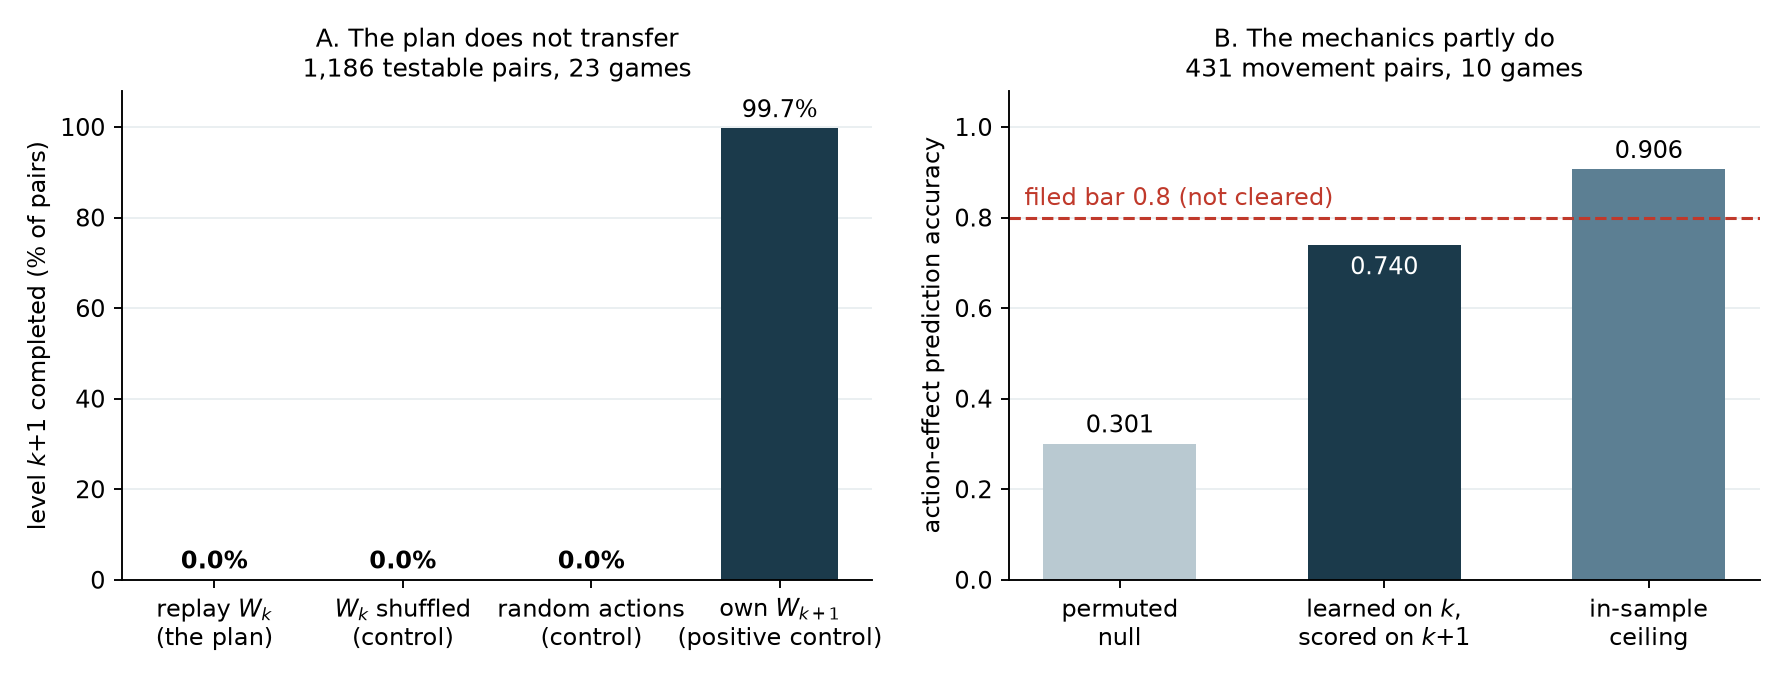
\includegraphics[width=1\linewidth,height=\textheight,keepaspectratio,alt={E21 results, drawn from experiments/E21\_level\_transfer.json by paper/make\_fig\_e21.py. Panel A: the share of testable pairs in which level k\{+\}1 is completed, over 1,186 pairs from 23 games (tn36 excluded because its positive control fails). Replaying W\_k, a shuffled W\_k and random actions complete none; the level's own W\_\{k+1\} completes 99.7 percent. Panel B: the action-effect accuracy of a mechanics model learned on level k and scored on level k\{+\}1 (431 pairs in 10 movement games), against its permuted null (over the 421 of those pairs that have one; the mean on those 421 is 0.757) and its in-sample ceiling, with the 0.8 bar filed in advance, which it did not clear.}]{figures/fig6_e21_transfer.png}
\caption{E21 results, drawn from
\protect\texttt{experiments/E21\_level\_transfer.json} by
\protect\texttt{paper/make\_fig\_e21.py}. Panel A: the share of testable
pairs in which level \(k{+}1\) is completed, over 1,186 pairs from 23
games (tn36 excluded because its positive control fails). Replaying
\(W_k\), a shuffled \(W_k\) and random actions complete none; the
level's own \(W_{k+1}\) completes 99.7 percent. Panel B: the
action-effect accuracy of a mechanics model learned on level \(k\) and
scored on level \(k{+}1\) (431 pairs in 10 movement games), against its
permuted null (over the 421 of those pairs that have one; the mean on
those 421 is 0.757) and its in-sample ceiling, with the 0.8 bar filed in
advance, which it did not clear.}
\end{figure}

One of three predictions was met, and the failures matter more.
Replaying a plan completes nothing, with a working positive control. The
1,186 pairs rest on only 144 distinct (game, level) transitions, about
eight sessions each, so the interval is quoted at both units: the
Clopper-Pearson 95 percent upper bound on the replay success rate is
0.31 percent treating pairs as independent and 2.5 percent at transition
level (0 of 144). Both are far below the 10 percent bar. In the 452
pairs whose budget \(|W_k|\) is at least the next human solution's
length (113 distinct transitions) replay also completes none: the 95
percent upper bound is 0.81 percent over pairs and 3.2 percent over
transitions (\texttt{experiments/budget\_check.out},
\texttt{experiments/e21\_numbers.out}). In the other 734 the next human
solution is longer than \(|W_k|\), so a replay could complete the level
only in fewer actions than that human used; they stay in the 1,186 but
test transfer only if such a shorter solution exists. Successive winning
sequences are only slightly more alike than a shuffle (0.446 against
0.431, pooled over all 1,314 pairs; difference 0.015, session-cluster 95
percent interval 0.012 to 0.019, 2,000 resamples of sessions) and are
above it on 17 of the 20 games where a shuffle can differ; on five games
(lp85, r11l, s5i5, tn36, vc33) a shuffle leaves the score unchanged in
every pair, and on three (ls20, m0r0, tu93) similarity sits below it.
The plan has structure but cannot be replayed. That is what our harness
fork's \texttt{solved\_levels()} hands its model. Shuffled plans and
random actions also complete 0 percent. Replay fails alike in the 12
click-driven and the 11 movement-driven games of the 23.

\textbf{Caveats.} The positive control fails on all 51 tn36 pairs (and 3
lf52, 1 sc25), so M1 is quoted without tn36 (with it: 0 of 1,237,
control 95.6 percent, the filed run); s5i5 has no testable pair; six
other games record no movement, so M3 is silent there. 188 of 6,185
random-control runs (3.0 percent, all lf52) exceeded a 60-second budget,
filed before any affected session was scored: random sequences drive
lf52 into states whose step cost grows without bound. They are reported
as unevaluable, because counting them as failures would flatter P21a. M3
has data on 10 of the 12 movement games; three of them (tu93, wa30,
re86) hold 48 percent of its 431 pairs, which rest on 56 distinct
transitions. The pair mean 0.740 has a session-cluster 95 percent
interval of 0.687 to 0.791 (99 sessions, 2,000 resamples), below the 0.8
bar, and leaving out any one game gives a mean between 0.704 and 0.787.
The game-weighted mean (the unweighted mean of the ten per-game means)
is 0.682, with a game-cluster 95 percent interval of 0.46 to 0.86 (10
games, 2,000 resamples), which includes 0.8, so the shortfall shows over
pairs and sessions but is not resolved over games. Per game, M3 is 0.99
on dc22, 0.97 on g50t, 0.90 on re86, 0.89 on ls20 and tu93, and 0.75 on
sp80 and wa30, but 0.36 on tr87, 0.30 on m0r0 and 0.00 on cd82 (one
transition, 10 pairs); we have not diagnosed the three low games.

\section{5. Two agents}\label{two-agents}

\textbf{5a. Mechanics memory on and off (our explorer, public 25
development set).} Memory on scores 0.277 and clears 13 levels, off
0.227 and 11, on our local scorer, from one seed pair (seed 0, agent
version v5) with no interval for the difference.
\texttt{EXPERIMENT\_LOG.csv} in the released repository holds four
further memory-on runs on the same 25 games and 2,000-action budget:
seed 1 of the same v5 agent (0.283, 14 levels) and seeds 0, 2 and 3 of
the later v7 agent (0.280, 0.276 and 0.278; v7 also learns which moves
lose the game and keeps scenery and thin bars out of goal predicates).
All five memory-on scores lie between 0.276 and 0.283. Memory off was
run once on the public 25 (seed 0, v5), so the off arm has no seed
spread and the 0.050 gap has no interval. Level-1 cost is identical, as
it must be since nothing is carried into a first level, and a second
level is reached only with memory on.

\textbf{5b. \texttt{solved\_levels()} on and off (LLM harness, hidden
55).} The model is Intel/Qwen3.8-Flash-Next-W4A16-AutoRound (the Intel
base) in Franzen's Milestone-2 harness. The Intel notebooks mount the
weights as the Kaggle model
dfranzen/intel-qwen3.8-flash-next-w4a16-autoround (Transformers/default,
version 1), Franzen's upload of Intel's quantization, together with a
separate speculative-decoding draft checkpoint,
dfranzen/albucino-qwen3-8-flash-next-drafter (version 1); we did not
record a Hugging Face revision of the weights. Serving and sampling are
Franzen's settings {[}3{]}, set explicitly in our notebook
configurations: one RTX PRO 6000, at most 10 concurrent game streams, a
131,072-token (128 Ki) context window with at most 12,288 (12 Ki)
generated tokens per request, thinking enabled, temperature 0.7, top-p
0.95, top-k 20. A scored rerun runs on the competition's hardware under
its 9-hour notebook limit, shared by all 110 games, at no charge to the
entrant, and does not draw on the account's weekly GPU quota. A draw is
one scored rerun of a notebook on the 55 hidden games. The helper
variant (v2) was paired with its twin without the helper (v1), two draws
each, taken from 19 to 25 October (Table 2); a pair on the Swift base
(UkisAI Swift1.5 post-train) was dropped after its first draw scored
4.92. That pair was v6-swift (helper on) and v3-swift (helper off), and
the filed rule names it (v6 - v3); v3-swift, smoke-tested on two public
games, was never submitted for a scored rerun, and the draw plan dropped
both Swift variants after v6's draw. \texttt{HYPOTHESES.md} filed no
stopping rule for the number of draws. The draw plan in the harness
repository (\texttt{kaggle/plan.json}) set two draws per variant before
the first draw. On 26 October, after the draws so far had scored like
unmodified copies of the notebook, the plan was changed: a second helper
variant on the Intel base (v7i, level memory plus a note pinned at each
context drain), queued for two draws, was dropped and never ran on the
hidden games, and the remaining daily slots went to v1f from 27 October
and to v10 from 30 October, so those variants have three and four draws.
v2 differs from v1 in two ways: it adds an optional REPL call,
\texttt{solved\_levels()}, that the level-up message mentions once, and
it rewords the budget-bar line of the prompt
(\texttt{ARC3\_BAR\_GUIDANCE=budget}). Both arms keep Franzen's
level-transfer guidance, which already tells the model to reuse the
previous level's mechanics. We do not know how often v2's model called
the helper: the logs of scored reruns are not visible to entrants, so
the calls in its two scored draws (57477157 and 57575322) cannot be
counted. The comparison therefore tests the helper together with the
reworded line.

\begin{longtable}[]{@{}
  >{\raggedright\arraybackslash}p{(\linewidth - 12\tabcolsep) * \real{0.3621}}
  >{\raggedright\arraybackslash}p{(\linewidth - 12\tabcolsep) * \real{0.1034}}
  >{\raggedleft\arraybackslash}p{(\linewidth - 12\tabcolsep) * \real{0.1034}}
  >{\raggedleft\arraybackslash}p{(\linewidth - 12\tabcolsep) * \real{0.1034}}
  >{\raggedleft\arraybackslash}p{(\linewidth - 12\tabcolsep) * \real{0.1034}}
  >{\raggedleft\arraybackslash}p{(\linewidth - 12\tabcolsep) * \real{0.1034}}
  >{\raggedright\arraybackslash}p{(\linewidth - 12\tabcolsep) * \real{0.1207}}@{}}
\caption{Hidden-set draws (55 games each) by variant.}\tabularnewline
\toprule\noalign{}
\begin{minipage}[b]{\linewidth}\raggedright
variant
\end{minipage} & \begin{minipage}[b]{\linewidth}\raggedright
helper
\end{minipage} & \begin{minipage}[b]{\linewidth}\raggedleft
draw 1
\end{minipage} & \begin{minipage}[b]{\linewidth}\raggedleft
draw 2
\end{minipage} & \begin{minipage}[b]{\linewidth}\raggedleft
draw 3
\end{minipage} & \begin{minipage}[b]{\linewidth}\raggedleft
mean
\end{minipage} & \begin{minipage}[b]{\linewidth}\raggedright
kernel versions
\end{minipage} \\
\midrule\noalign{}
\endfirsthead
\toprule\noalign{}
\begin{minipage}[b]{\linewidth}\raggedright
variant
\end{minipage} & \begin{minipage}[b]{\linewidth}\raggedright
helper
\end{minipage} & \begin{minipage}[b]{\linewidth}\raggedleft
draw 1
\end{minipage} & \begin{minipage}[b]{\linewidth}\raggedleft
draw 2
\end{minipage} & \begin{minipage}[b]{\linewidth}\raggedleft
draw 3
\end{minipage} & \begin{minipage}[b]{\linewidth}\raggedleft
mean
\end{minipage} & \begin{minipage}[b]{\linewidth}\raggedright
kernel versions
\end{minipage} \\
\midrule\noalign{}
\endhead
\bottomrule\noalign{}
\endlastfoot
v2-level-memory & on & 29.54 & 19.75 & & 24.65 & 2, 4 \\
v1-franzen-faithful & off & 29.93 & 25.85 & & 27.89 & 2, 5 \\
v1f (v1 code, faster model load) & off & 29.44 & 21.86 & 28.19 & 26.50 &
1 \\
\end{longtable}

Leaderboard scores of first-time copies of the reference notebook
(hundreds of teams, one draw each; the thread gives no sample size and
does not say whether every copy was unedited or whether failed runs were
dropped) have mean 25.77, standard deviation (SD) 3.93 {[}21{]}, and an
independent study reports SD 3.99 over ten evaluations of one frozen
harness on twenty public games {[}22{]}; two single draws therefore
differ with SD about 5.5. The rule filed before any pair ran claims an
effect only above 11 points, twice that, and predicted none. The means
of the v2 and v1 arms differ by 3.2 (0.8 SD, where 3.93 is the SD of a
difference between two-draw means), the helper arm lower. No effect is
claimed; two draws per arm resolve only 11 points (the 95 percent
interval for off minus on runs from \(-4.5\) to \(+10.9\)), so the data
leave an effect of either sign open. Pooling the three v1f draws with v1
gives five draws without the helper: mean 27.05, SD 3.30, 2.4 points
above the helper arm. As of 2 November, all thirteen valid Intel draws,
across five variants (v1, v1f, v2, v8i, which is v1 plus a slot-priority
rule called D' in our logs, and v10, which is v1f plus start-up
hardening and three harness fixes: a guarded RESET, a notice after
cut-off replies, and attempt-loss stops), average 26.35 (SD 3.18),
indistinguishable from an unmodified copy of the notebook we forked. The
draws not in Table 2 are 24.95 and 26.47 (v8i, kernel versions 1 and 3)
and 24.51, 29.78, 27.60 and 24.72 (v10, version 1).

Two earlier draws, one per arm (22 and 23 October), returned 0.00 and
are excluded from every count and mean. We attribute them to the
platform ending a rerun after 15 minutes without a game move, together
with slower model loading, so they say nothing about either arm. Both
arms were redrawn after a keepalive fix: a game reset sent every five
minutes until the model server is ready.

\section{6. The floor and the hidden
ranking}\label{the-floor-and-the-hidden-ranking}

Contact curiosity is a term in the explorer's planner that prefers
states where the mover touches a rarely contacted object class. Table 3
sets the hidden score of each explorer submission beside the public-set
score of its nearest measured twin.

\begin{longtable}[]{@{}llll@{}}
\caption{Explorer submissions, hidden score against the nearest measured
public-set score.}\tabularnewline
\toprule\noalign{}
submission & agent & public 25 (nearest measured twin) & hidden 55 \\
\midrule\noalign{}
\endfirsthead
\toprule\noalign{}
submission & agent & public 25 (nearest measured twin) & hidden 55 \\
\midrule\noalign{}
\endhead
\bottomrule\noalign{}
\endlastfoot
57095368 & explorer, crashed to cyclic fallback & n/a & 0.15 \\
57170721 & random, 60 actions/game & n/a & 0.12 \\
57123503 & explorer, memory on & 0.280 & 0.08 \\
57199354 & explorer, memory off & 0.227 (v5 twin) & 0.08 \\
57248168 & explorer, contact curiosity off & 0.204 (v4 twin) & 0.01 \\
\end{longtable}

The first four rows suggest the hidden metric ignores the agent: a
random agent outscores the working one, and a memory switch worth
\(+0.050\) publicly (the v5 pair, 0.277 against 0.227) is worth 0.000
here. The fifth row differs by about one level: with contact curiosity
off, the explorer scores 0.01 against 0.08 on the hidden 55 in one draw
each (0.07 \(\times\) 55 = 3.9 points). Contact curiosity is worth
\(+0.080\) publicly on the v4 pair, all of it from one game, lp85;
without lp85 the contact-on agent scores lower than the contact-off
agent on the public 25.

Contact curiosity is consistent with a gain in first-level efficiency:
it cuts median level-1 cost from 21.2 to 8.6 times the human cost
(medians over 10 and 11 games; on the nine games the two sets share,
21.95 against 8.59 times; \texttt{experiments/level1\_cost\_check.out}),
and the hidden metric squares that ratio. Memory is consistent with
later-level coverage, a second level on two more games, which the metric
nearly ignores. Here the hidden ranking says little about this paper's
treatment. Three public games supply 90 percent of our public 0.280, the
hidden 0.08 sums to 4.4 points over 55 games (0.08 \(\times\) 55),
roughly one such level, and on 13 October 1,087 of 4,233 teams sat in
the (0.05, 0.23{]} band that contains our 0.08.

\section{7. Limitations and scope}\label{limitations-and-scope}

Scope: one benchmark (ARC-AGI-3), human replays on the public 25 games
only, one LLM base model (a second pair was dropped); nothing here tests
transfer outside ARC-AGI-3. The replay test (M1) needs only recorded
multi-level sessions, a deterministic replayable build and a
level-completion signal, so it could be repeated on other game suites
whose levels reuse mechanics; we ran it on one.

\textbf{Contamination, agent view and outcomes.} The 55 games behind the
harness draws are the half of the competition's hidden games whose
aggregate score the public leaderboard shows, and the same 55 were
scored on every draw; the final ranking uses the other half. We know of
no public release of these games and did not test whether the model had
seen them. The explorer was developed on the public 25 games, so 5a is
development-set evidence; its hidden scores are in Table 3. For the
harness arms, the \texttt{arc\_agi} 0.9.8 package that the notebooks
install does not serve the human baseline action counts in its game
listings, but we did not audit the model's Python sandbox for other
information about the hidden games, and the logs of scored reruns are
not visible to entrants, so we have not read the model's view of any
hidden game. The only outcome available for a hidden draw is its
aggregate score. We therefore report no solved, partly solved or failed
outcomes per game or level for the harness arms and no counts of tool or
harness failures (timeouts, replies cut off at the output limit, lost
attempts); the only failures reported are the two 0.00 draws attributed
to the platform. For the explorer, 5a gives the score and the number of
levels cleared, not per-game outcomes.

The effect model expresses only rigid displacements, so the explorer
memorises click and recolour mechanics and cannot plan toward them;
outside the template class, mechanics memory gives nothing. The LLM arm
has two draws per variant against a 3.93-point copy spread, its second
draws ran with slower model loading, and the two draws of each arm ran
on different kernel versions. E21 measures human play, so it bounds what
is available to transfer and says nothing about what an agent uses. M1
tests a verbatim replay within the budget \(|W_k|\). A model that adapts
a plan it is shown can do things M1 does not test, and 330 of the 1,237
sequences \(W_k\) are longer than the 60 actions the harness shows.

Other filed predictions mostly failed. The explorer's level-1 efficiency
(P1) and next-state accuracy (P4) predictions were not met. The
click-effect (E12), ordered-goal (E13) and first goal-proposer (E19)
extensions were negative. The proposer follow-ups gained about 0.015 on
the public 25 and replicated (E20 and E20b with one proposer, E20c with
another). E20c with the first proposer lost a game, and E20d failed its
gate. All are in \texttt{HYPOTHESES.md}.

\section{8. Conclusion}\label{conclusion}

Replaying a winning plan verbatim completes no next level in human play,
and the harness arm with the plan-returning helper, which also had a
reworded prompt line, averaged 3.2 points below its twin over two draws
each, inside the draw noise. Mechanics predict next-level movement at
0.740, short of the bar we filed, though predicting a move is not
solving a level. For anyone aiming at 85 percent, later levels must be
cheap, and verbatim replay did not supply them; a replay that adapts the
plan is untested. Next entrants should log that a feature is used before
crediting it, and report several draws against the copy spread.

\section{Linked competition
submission}\label{linked-competition-submission}

57477157 (\texttt{v2-level-memory}, kernel version 2): Franzen's
Milestone-2 harness plus \texttt{solved\_levels()} and a reworded
budget-bar line; 29.54 hidden, the better of two draws and one SD above
our 13-draw Intel mean, so expect a private score nearer 26.

\section{Code and data}\label{code-and-data}

\begingroup\raggedright

Code, data and every experiment log are released with the paper, at
commit cb494af of arc-prize-2026 and commit 662b680 of arc-agi-3; the
paths below are those of these commits.

\begin{itemize}
\tightlist
\item
  \url{https://github.com/rodriguescarson/arc-prize-2026} holds the
  explorer (\texttt{src/arc\_prize\_2026/arc3/agents/model\_based.py}),
  the replay code
  (\texttt{src/arc\_prize\_2026/arc3/level\_transfer.py}, tested by
  \texttt{tests/test\_level\_transfer.py}), the 340 replay sessions in
  packed form (\texttt{data/human\_replays\_packed}, terms in its
  \texttt{NOTICE}), \texttt{EXPERIMENT\_LOG.csv} and
  \texttt{submission/SUBMISSIONS.md}.
\item
  Its folder \texttt{paper/level-transfer} holds \texttt{HYPOTHESES.md},
  the figure, the experiment outputs, \texttt{CLAIM-MAP.md} (the source
  file of each number) and the scripts that regenerate the numbers of
  Sections 4 and 5b and the level-1 costs of Section 6
  (\texttt{experiments/e21\_numbers.py},
  \texttt{experiments/hidden\_draws.py},
  \texttt{experiments/budget\_check.py},
  \texttt{experiments/level1\_cost\_check.py}). The other numbers of
  Sections 5a and 6 are read from \texttt{EXPERIMENT\_LOG.csv},
  \texttt{submission/SUBMISSIONS.md} and the per-run
  \texttt{results.json} files under the repository-root
  \texttt{experiments/} folder.
\item
  \url{https://github.com/rodriguescarson/arc-agi-3} holds the harness
  fork
  (\texttt{harness/ARC3-Inference/inference/utils/level\_memory.py}),
  the notebook builder and its cells
  (\texttt{kaggle/build\_notebook.py}, \texttt{kaggle/cells/}), the
  variant configurations (\texttt{kaggle/variants/}) and its submission
  log (\texttt{docs/SUBMISSIONS.md}).
\end{itemize}

\par\endgroup

\section{Disclosure}\label{disclosure}

Competing interests: the author is an entrant in the ARC Prize 2026
ARC-AGI-3 competition on Kaggle, which awards cash prizes, and the
linked submission was scored in it. An earlier version of this paper was
submitted to the competition's Paper Track, which also awards cash
prizes.

Funding: this work received no external funding.

Data rights: the replay sessions come from the ARC Prize human-testing
release {[}20{]}. Neither the release post nor its Hugging Face mirror
names a licence; both call the data open source. The
\texttt{arc-prize-2026} repository's
\texttt{data/human\_replays\_packed} redistributes the mirror's 340
sessions repacked as NumPy files (the frames, actions, per-step level
counts and game states of one session, with its environment and session
identifiers and no timestamps). Its NOTICE states that these files are
not covered by the repository's MIT-0 licence and keep the terms of the
original release; we grant no licence to them and make no claim about
what the source permits. We did not review the sessions for personal
data.

Claude Code (Anthropic) wrote most of the code, ran the experiments and
drafted this text under the author's direction. The author set the
hypotheses and the filed predictions, reviewed every change and approved
each claim; every number from our own runs comes from the released code
or the Kaggle submission list and traces to a file in the repository;
numbers from other sources are cited, except the 13 October leaderboard
count in Section 6, which comes from a public leaderboard download that
is not redistributed.

\section{References}\label{references}

\begin{enumerate}
\def\labelenumi{\arabic{enumi}.}
\tightlist
\item
  ARC Prize Foundation. ARC-AGI-3: A New Challenge for Frontier Agentic
  Intelligence. arXiv:2603.24621,
  \url{https://arxiv.org/abs/2603.24621}, 2026.
\item
  Tufa Labs. The Duck harness, winning solution to ARC-AGI-3 Milestone
  1. \url{https://github.com/Tufalabs/duck-harness}, 2026.
\item
  D. Franzen. ARC-AGI-3 Milestone 2 solution.
  \url{https://github.com/da-fr/arc-agi-3-solution}, 2026 (Kaggle
  notebook
  \url{https://www.kaggle.com/code/dfranzen/arc-agi-3-milestone-2-solution}).
\item
  rellik13 (Kaggle user sirikilohit). arc-agi-3-duck-18-1gc-submit.
  Kaggle notebook,
  \url{https://www.kaggle.com/code/sirikilohit/arc-agi-3-duck-18-1gc-submit},
  2026.
\item
  D. Smit. StochasticGoose.
  \url{https://github.com/DriesSmit/ARC3-solution}, 2025.
\item
  nihilisticneuralnet. {[}0.46{]} ARC-AGI-3: Persistent Memory BFS ARC
  Solver. Kaggle notebook,
  \url{https://www.kaggle.com/code/nihilisticneuralnet/0-46-arc-agi-3-persistent-memory-bfs-arc-solver},
  2026.
\item
  J. Lehmann, A. Aioanei, S. Vahdati. Tycho: Active Abstraction with
  Programmatic World Models for ARC-AGI-3. arXiv:2607.28287,
  \url{https://arxiv.org/abs/2607.28287}, 2026.
\item
  A. Skoutnev et al.~Twin: Playing an Unknown Game with a Test-Time
  Digital Twin. arXiv:2608.14490,
  \url{https://arxiv.org/abs/2608.14490}, 2026.
\item
  A. Fox et al.~PRO-LONG: Programmatic Memory Enables Long-Horizon
  Reasoning. arXiv:2607.20064, \url{https://arxiv.org/abs/2607.20064},
  2026.
\item
  G. Zeng et al.~Schema: Discovering Unknown Environments via Agentic
  Program Induction. arXiv:2609.39140,
  \url{https://arxiv.org/abs/2609.39140}, 2026.
\item
  Q. Han et al.~VISTA: A Visual Harness for Reasoning in an Interactive
  World. arXiv:2610.02200, \url{https://arxiv.org/abs/2610.02200}, 2026.
\item
  H. Zhao et al.~Memento 3: Model-Based Recursive Self-Improvement
  through Reflective Rulebooks. arXiv:2610.11794,
  \url{https://arxiv.org/abs/2610.11794}, 2026.
\item
  W. Wu. Kepler: Auditable World Models for ARC-AGI-3. arXiv:2610.00834,
  \url{https://arxiv.org/abs/2610.00834}, 2026.
\item
  K. H. Liew. Explore Before You Solve: The Speed-Depth Trade-off in
  Epistemic Agents for ARC-AGI-3. arXiv:2605.25931,
  \url{https://arxiv.org/abs/2605.25931}, 2026.
\item
  P. Furgale et al.~NVIDIA-labs OO Agents: Native Python Object-Oriented
  Agents. arXiv:2607.20709, \url{https://arxiv.org/abs/2607.20709},
  2026.
\item
  C. Wu, J. Passenger, Y. Song. Tracing the Thoughts of a Coding Agent
  Playing ARC-AGI-3: Lessons for Continual Learning. arXiv:2610.11450,
  \url{https://arxiv.org/abs/2610.11450}, 2026.
\item
  R. Lencevicius. When the harness decides success: state that cannot be
  re-observed. arXiv:2610.26632, \url{https://arxiv.org/abs/2610.26632},
  2026.
\item
  S. Liu et al.~How Humans Learn Unfamiliar Worlds: A Think-Aloud
  Dataset on ARC-AGI-3. arXiv:2610.34523,
  \url{https://arxiv.org/abs/2610.34523}, 2026.
\item
  E. Akyürek et al.~The Surprising Effectiveness of Test-Time Training
  for Few-Shot Learning (the ARC Prize 2024 results list it as
  ``\ldots{} for Abstract Reasoning''). arXiv:2411.07279,
  \url{https://arxiv.org/abs/2411.07279}, 2024.
\item
  G. Kamradt (ARC Prize). Measuring Human Performance on ARC-AGI-3.
  \url{https://arcprize.org/blog/arc-agi-3-human-dataset}, 14 April 2026
  (Hugging Face mirror by magic-sword:
  \url{https://huggingface.co/datasets/magic-sword/arc_agi_3_public_demo_human_testing}).
\item
  S. Pham. Incredible notebook performance variation (Daniel Franzen's
  copies data analysis). Kaggle discussion 745062,
  \url{https://www.kaggle.com/discussions/general/745062}, October 2026.
\item
  J. Lehmann, S. Vahdati. Can LLMs Improve Their Own Harness? A
  Controlled Study on ARC-AGI-3. arXiv:2610.30499,
  \url{https://arxiv.org/abs/2610.30499}, 2026.
\end{enumerate}

\end{document}
